% !Mode:: "TeX:UTF-8"

%%%%%%%%%%%%%%%%% Fonts Definition and Basics %%%%%%%%%%%%%%%%%
% 宋体
\setCJKfamilyfont{song}{SimSun}
\newcommand{\song}{\CJKfamily{song}}
% 仿宋体
\setCJKfamilyfont{fs}{FangSong_GB2312}
\newcommand{\fs}{\CJKfamily{fs}}
% 楷体
\setCJKfamilyfont{kai}{KaiTi_GB2312}
\newcommand{\kai}{\CJKfamily{kai}}
% 黑体
\setCJKfamilyfont{hei}{SimHei}
\newcommand{\hei}{\CJKfamily{hei}}
% 隶书
\setCJKfamilyfont{li}{LiSu}
\newcommand{\li}{\CJKfamily{li}}

\newcommand{\chuhao}{\fontsize{28pt}{28pt}\selectfont}       % 初号, 单倍行距
\newcommand{\yihao}{\fontsize{26pt}{26pt}\selectfont}       % 一号, 单倍行距
\newcommand{\xiaoyi}{\fontsize{24pt}{24pt}\selectfont}      % 小一, 单倍行距
\newcommand{\erhao}{\fontsize{22pt}{1.25\baselineskip}\selectfont}       % 二号, 1.25倍行距
\newcommand{\xiaoer}{\fontsize{18pt}{18pt}\selectfont}      % 小二, 单倍行距
\newcommand{\sanhao}{\fontsize{16pt}{16pt}\selectfont}      % 三号, 单倍行距
\newcommand{\xiaosan}{\fontsize{15pt}{15pt}\selectfont}     % 小三, 单倍行距
\newcommand{\sihao}{\fontsize{14pt}{14pt}\selectfont}       % 四号, 单倍行距
\newcommand{\xiaosi}{\fontsize{12pt}{12pt}\selectfont}      % 小四, 单倍行距
\newcommand{\wuhao}{\fontsize{10.5pt}{10.5pt}\selectfont}   % 五号, 单倍行距
\newcommand{\xiaowu}{\fontsize{9pt}{9pt}\selectfont}        % 小五, 单倍行距

% 重新定义了波浪符~的意义
% ctex 在 CJK 环境里自动使用 \CJKtilde???
%\CJKtilde

% 定义章的pre-post名称:第 n 章
\newcommand\prechaptername{第}
\newcommand\postchaptername{章}

% 调整中文字符的表示,行内占一个字符宽度,行尾占半个字符宽度
% 行末半角?
\punctstyle{hangmobanjiao}

% 调整罗列环境的布局
\setitemize{leftmargin=3em,itemsep=0em,partopsep=0em,parsep=0em,topsep=-0em}
\setenumerate{leftmargin=3em,itemsep=0em,partopsep=0em,parsep=0em,topsep=0em}

% 避免宏包 hyperref 和 arydshln 不兼容带来的目录链接失效的问题。
\def\temp{\relax}
\let\temp\addcontentsline
\gdef\addcontentsline{\phantomsection\temp}

% 自定义项目列表标签及格式 \begin{publist} 列表项 \end{publist}
\newcounter{pubctr} %自定义新计数器
\newenvironment{publist}{%%%%%定义新环境
\begin{list}{[\arabic{pubctr}]} %%标签格式
    {
     \usecounter{pubctr}
     \setlength{\leftmargin}{2.5em}   % 左边界 \leftmargin =\itemindent + \labelwidth + \labelsep
     \setlength{\itemindent}{0em}     % 标号缩进量
     \setlength{\labelsep}{1em}       % 标号和列表项之间的距离,默认0.5em
     \setlength{\rightmargin}{0em}    % 右边界
     \setlength{\topsep}{0ex}         % 列表到上下文的垂直距离
     \setlength{\parsep}{0ex}         % 段落间距
     \setlength{\itemsep}{0ex}        % 标签间距
     \setlength{\listparindent}{0pt}  % 段落缩进量
    }}
{\end{list}}

%makeatletter --> makeatother: \makeatletter使得@成为一个普通字母
\makeatletter
	\renewcommand\normalsize{
		\@setfontsize\normalsize{12pt}{12pt} % 小四对应 12 pt
		\setlength\abovedisplayskip{4pt}
		\setlength\abovedisplayshortskip{4pt}
		\setlength\belowdisplayskip{\abovedisplayskip}
		\setlength\belowdisplayshortskip{\abovedisplayshortskip}
		\let\@listi\@listI}
	
	% 不同的行距设置
	% TJU原始值1.63
	% 设为1.8则一页31行,1.95则一页29行(目前采用值)
	\def\defaultfont{\renewcommand{\baselinestretch}{1.95}\normalsize\selectfont} % 设置行距,正文一页29行
	
	% 控制字间距,使每行 34 个汉字
	\renewcommand{\CJKglue}{\hskip -0.1 pt plus 0.08\baselineskip}
\makeatother

%%%%%%%%%%%%% Contents 目录 %%%%%%%%%%%%%%%%%
\renewcommand{\contentsname}{目\qquad 录}
% 控制目录深度(目录页排版只排到二级标题,即章和节),改为1
\setcounter{tocdepth}{1}
\titlecontents{chapter}[2em]{\vspace{.0\baselineskip}\sihao\song}	% 可以重调skip
	{\prechaptername~\thecontentslabel~\postchaptername\quad}{}
	{\!\titlerule*[5pt]{$\cdot$}\!\!\!\!\sihao\contentspage}	% 调整点的距离
\titlecontents{section}[3em]{\vspace{-0.1\baselineskip}\xiaosi\song}
	{\thecontentslabel\quad}{}
	{\!\titlerule*[5pt]{$\cdot$}\!\!\!\!\xiaosi\contentspage}
\titlecontents{subsection}[4em]{\vspace{-0.2\baselineskip}\wuhao\song}
	{\thecontentslabel\quad}{}
	{\!\titlerule*[5pt]{$\cdot$}\!\!\!\!\wuhao\contentspage}


%%%%%%%%%% Chapter and Section 章节 %%%%%%%%%%%%%
\setcounter{secnumdepth}{4}
% 设置段落间距
\setlength{\parindent}{2em}

% 如果使用第“一”章
%\renewcommand{\chaptername}{\prechaptername\CJKnumber{\thechapter}\postchaptername}
% 使用第“1”章
\renewcommand{\chaptername}{\prechaptername~\thechapter~\postchaptername}

%\titleformat{command}[shape]{format}{label}{sep}{before}[after]
% 此处修改的chapter title会被主文件定义覆盖
% chapter标题格式:小二,黑体,居中
\titleformat{\chapter}{\centering\xiaoer\hei}{}{2em}{}
\titlespacing{\chapter}{0pt}{0.1\baselineskip}{0.8\baselineskip}
% section标题格式:小三,宋体加粗,左对齐
\titleformat{\section}{\xiaosan\song\bfseries}{}{1em}{\thesection \quad}
\titlespacing{\section}{0pt}{0.15\baselineskip}{0.25\baselineskip}
% subsection标题格式:四号,宋体加粗,左对齐
\titleformat{\subsection}{\sihao\song\bfseries}{}{1em}{\thesubsection \quad}
\titlespacing{\subsection}{0pt}{0.1\baselineskip}{0.3\baselineskip}
% subsubsection标题格式:小四,宋体加粗,左对齐
\titleformat{\subsubsection}{\xiaosi\song\bfseries}{}{1em}{\thesubsubsection \quad}
\titlespacing{\subsubsection}{0pt}{0.05\baselineskip}{0.1\baselineskip}


%%%%%%%%%% Table, Figure and Equation 图/表/公式 %%%%%%%%%%%%%%%%%
\renewcommand{\tablename}{表}
\renewcommand{\figurename}{图}
% 使图编号为 7-1 的格式
\renewcommand{\thefigure}{\arabic{chapter}-\arabic{figure}}
% 使子图编号为 a) 的格式
\renewcommand{\thesubfigure}{\alph{subfigure}}
% 使子图编号为 (a) 的格式
%\renewcommand{\thesubfigure}{(\alph{subfigure})}
% 使子表编号为 (a) 的格式
\renewcommand{\thesubtable}{(\alph{subtable})}
% 使表编号为 7-1 的格式
\renewcommand{\thetable}{\arabic{chapter}-\arabic{table}}
% 使公式编号为 7-1 的格式
\renewcommand{\theequation}{\arabic{chapter}-\arabic{equation}}
\makeatletter
	% 使子图引用也是7-1a)或7-1(a)的形式
	\renewcommand{\p@subfigure}{\thefigure}
\makeatother
% 定制浮动图形和表格标题样式
\makeatletter
	\long\def\@makecaption#1#2{
	   \vskip\abovecaptionskip
	   \sbox\@tempboxa{\centering\wuhao\song{#1\quad #2}}
	   % 控制图片说明对齐方式:单行居中/多行左对齐
	   \ifdim \wd\@tempboxa >\hsize
	     \flushleft\wuhao\song{#1\quad #2} \par	% narrower
	   \else
	     \global \@minipagefalse
	     \hb@xt@\hsize{\hfil\box\@tempboxa\hfil}
	   \fi
	   \vskip\belowcaptionskip}
\makeatother
% 用来控制longtable表头分隔符(依赖于subfigure)
%\captiondelim{~~~~}


%%%%%%%%%% Theorem Environment 定理 %%%%%%%%%%%%%%%%%
\theoremstyle{plain}
\theorembodyfont{\song\rmfamily}
\theoremheaderfont{\hei\rmfamily}
\newtheorem{theorem}{定理~}[chapter]
\newtheorem{lemma}{引理~}[chapter]
\newtheorem{axiom}{公理~}[chapter]
\newtheorem{proposition}{命题~}[chapter]
\newtheorem{prop}{性质~}[chapter]
\newtheorem{corollary}{推论~}[chapter]
\newtheorem{conclusion}{结论~}[chapter]
\newtheorem{definition}{定义~}[chapter]
\newtheorem{conjecture}{猜想~}[chapter]
\newtheorem{example}{例~}[chapter]
\newtheorem{remark}{注~}[chapter]
%\newtheorem{algorithm}{算法~}[chapter]
\newenvironment{proof}{\noindent{\hei 证明:}}{\hfill $ \square $ \vskip 4mm}
\theoremsymbol{$\square$}


%%%%%%%%%% 伪代码 %%%%%%%%%%%%%%%%%
%\floatname{algorithm}{算法}
%\renewcommand{\algorithmicrequire}{\textbf{输入:}}
%\renewcommand{\algorithmicensure}{\textbf{输出:}}


%%%%%%%%%% Page: number, header and footer 页面设置 %%%%%%%%%%%%%%%%%
%\frontmatter 或 \pagenumbering{roman}
%\mainmatter 或 \pagenumbering{arabic}
\makeatletter
	\renewcommand\frontmatter{\clearpage
		\@mainmatterfalse}
\makeatother


%%%%%%%%%%%% References 参考文献 %%%%%%%%%%%%%%%%%
\renewcommand{\bibname}{参考文献}
% 重定义参考文献样式,来自thu
\makeatletter
	\renewenvironment{thebibliography}[1]{
    %\titleformat{\chapter}{\raggedright\sihao\hei}{\chaptername}{2em}{}
    %\titleformat{\chapter}{\centering\sihao\hei}{\chaptername}{2em}{}
    %\titleformat{\chapter}{\centering\xiaoer\hei}{\chaptername}{2em}{}
   \chapter*{\bibname}
   \wuhao
   \list{\@biblabel{\@arabic\c@enumiv}}
        {\renewcommand{\makelabel}[1]{##1\hfill}
         \settowidth\labelwidth{0 cm}
         \setlength{\labelsep}{0pt}
         \setlength{\itemindent}{0pt}
         \setlength{\leftmargin}{\labelwidth+\labelsep}
         \addtolength{\itemsep}{-0.7em}
%         \addtolength{\itemsep}{-1.0em}
         \linespread{1.5}\selectfont	% 调整每个参考文献项内的间距 !!!
         \usecounter{enumiv}
         \let\p@enumiv\@empty
         \renewcommand\theenumiv{\@arabic\c@enumiv}}
    \sloppy\frenchspacing
    \clubpenalty4000
    \@clubpenalty \clubpenalty
    \widowpenalty4000
    \interlinepenalty4000
    \sfcode`\.\@m}
   {\def\@noitemerr
     {\@latex@warning{Empty `thebibliography' environment}}
    \endlist\frenchspacing}
\makeatother
% 缩小参考文献间的垂直间距
\addtolength{\bibsep}{-0.5em}
% 每个条目自第二行起缩进的距离
\setlength{\bibhang}{2em}

% 引用格式
\bibpunct{[}{]}{,}{s}{}{,}
% 默认参考文献引用号与正文内容一直,[]包裹
\citestyle{plain}
% 参考文献引用号作为上标出现
\newcommand{\supercite}[1]{\textsuperscript{\cite{#1}}}

%%%%%%%%%%%% Cover 封面、摘要、版权、致谢格式定义 %%%%%%%%%%%%%%%%%
\makeatletter % 一直到结尾
	\def\ctitle#1{\def\@ctitle{#1}}\def\@ctitle{}
	\def\etitle#1{\def\@etitle{#1}}\def\@etitle{}
	\def\csubject#1{\def\@csubject{#1}}\def\@csubject{}
	\def\esubject#1{\def\@esubject{#1}}\def\@esubject{}
	\def\cauthor#1{\def\@cauthor{#1}}\def\@cauthor{}
	\def\eauthor#1{\def\@eauthor{#1}}\def\@eauthor{}
	\def\csupervisor#1{\def\@csupervisor{#1}}\def\@csupervisor{}
	\def\esupervisor#1{\def\@esupervisor{#1}}\def\@esupervisor{}
	\def\cdate#1{\def\@cdate{#1}}\def\@cdate{}
	\long\def\cabstract#1{\long\def\@cabstract{#1}}\long\def\@cabstract{}
	\long\def\eabstract#1{\long\def\@eabstract{#1}}\long\def\@eabstract{}
	\def\ckeywords#1{\def\@ckeywords{#1}}\def\@ckeywords{}
	\def\ekeywords#1{\def\@ekeywords{#1}}\def\@ekeywords{}
	\def\cheading#1{\def\@cheading{#1}}\def\@cheading{}
	
	%TODO 页眉页脚设置	
	\renewcommand{\chaptermark}[1]%
	{\markboth{\chaptername \ #1}{}}            % \chaptermark 去掉章节标题中的数字
	\renewcommand{\sectionmark}[1]%
	{\markright{\thesection \ #1}{}}            % \sectionmark 去掉章节标题中的数字
	\fancypagestyle{newfancy}{
		\fancyhf{}
		% 左页眉,\rightmark 在 article 中包含 subsection 信息,在 report 和 book 中包含 section 信息
		\lhead{\song\wuhao \@ctitle}
%		%\lhead{\song\wuhao \@cheading}
		% 右页眉,\leftmark 在 article 中包含section的信息,在 report 和 book 中包含 chapter 的信息
		\rhead{\song\wuhao \leftmark}
		%\rhead{\prechaptername~\thechapter~\postchaptername}
		\renewcommand{\headrulewidth}{0.5 pt}
		\fancyfoot[C]{\song\xiaowu ~\thepage~}
	}

	\newlength{\@title@width}

	%TODO 定义封面
	\def\makecover{
	\phantomsection
	\pdfbookmark[-1]{\@ctitle}{ctitle}
	
	\ifsubmit
		\begin{titlepage}
			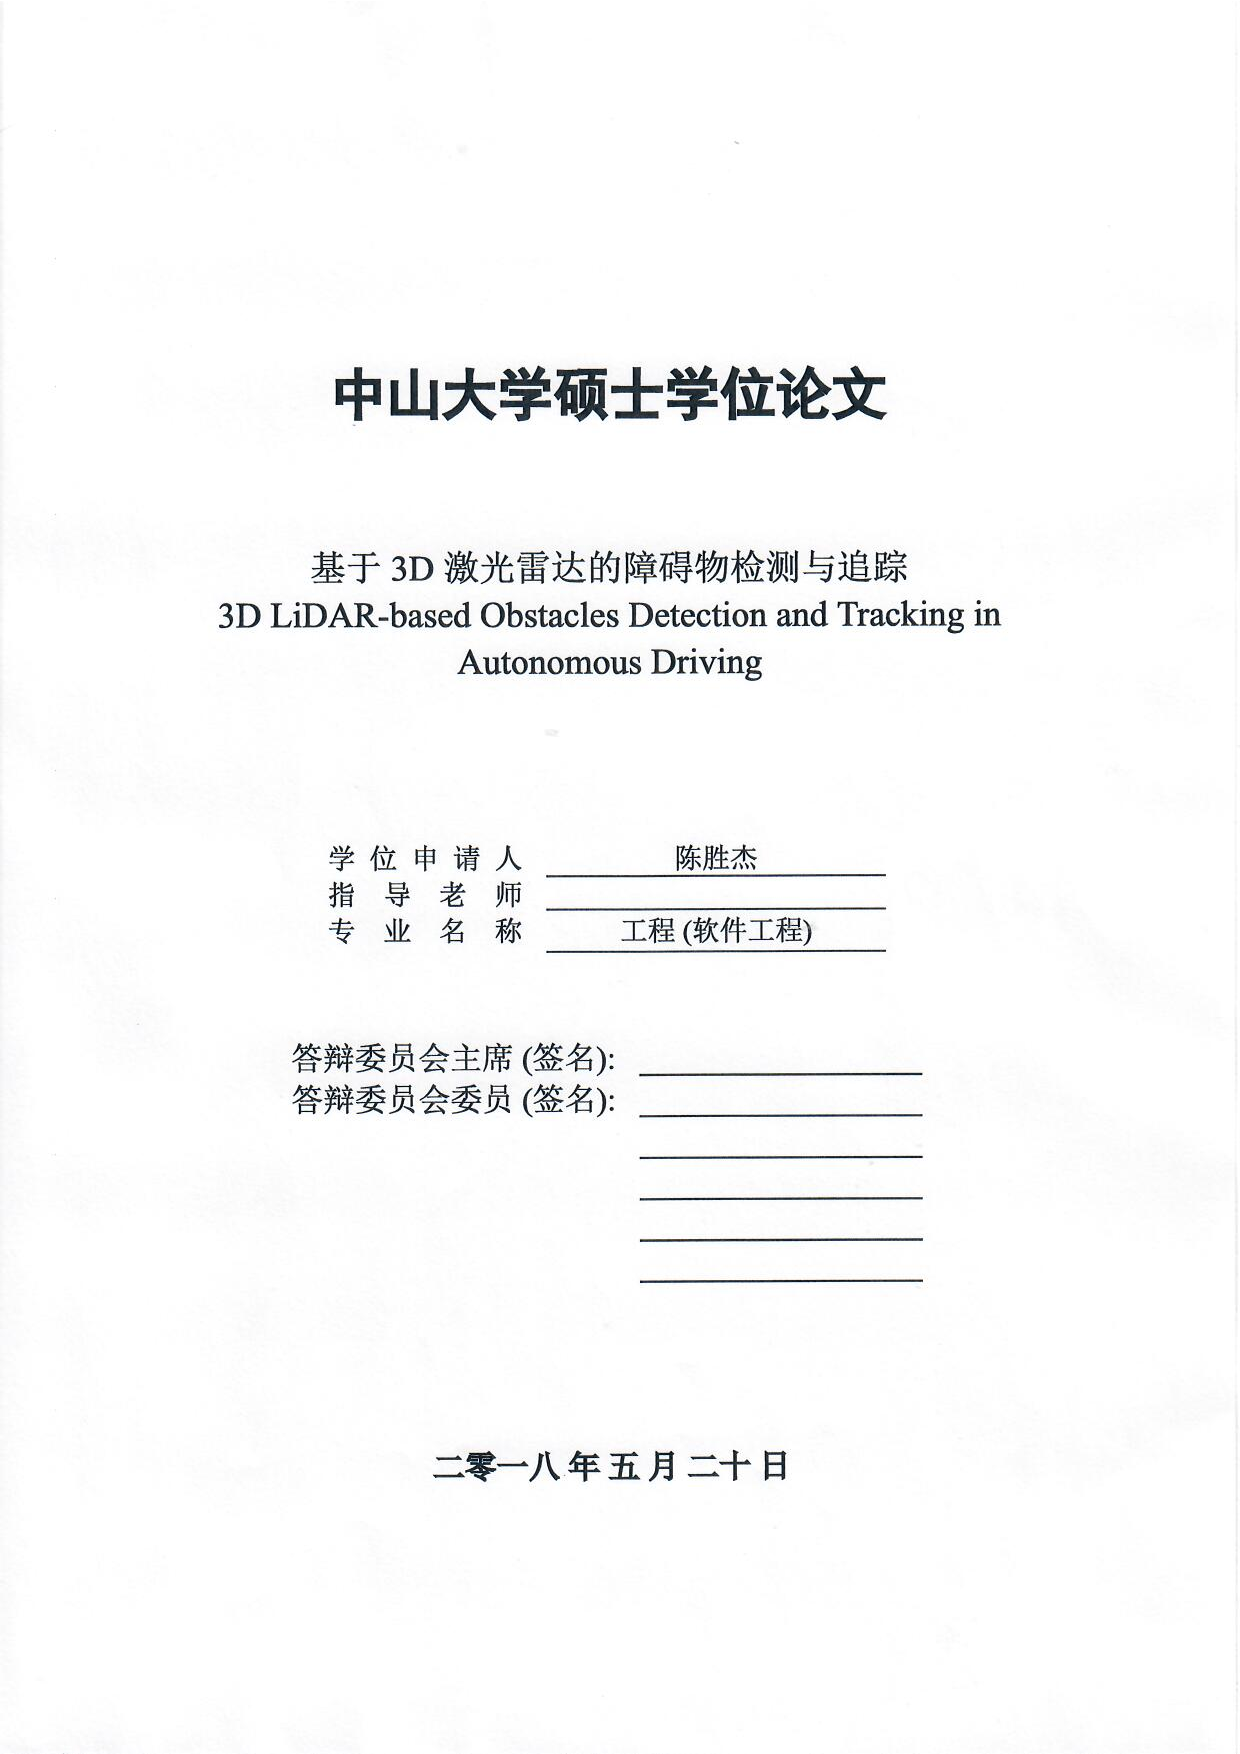
\includepdf{./signatures/TitlePage.pdf}
		\end{titlepage}	
	\else
		\begin{titlepage}
			\vspace*{31.5pt}
			\begin{center}
		
			\vspace*{21pt}
			\hei\chuhao{\textbf{中山大学硕士学位论文}}
		
			\vspace*{60pt}
			\song\xiaoer{\@ctitle}
		
			\xiaoer{\textrm{\@etitle}}
		
			\vspace*{80pt}
			\setlength{\@title@width}{6cm}	% 控制封面中下划线的长度。
			{\sihao\song{
			\begin{tabular}{lc}
			 学~~位~~申~~请~~人   &  \underline{\makebox[\@title@width][c]{\@cauthor}} \\
			 指~~~~导~~~~老~~~~师       &  \underline{\makebox[\@title@width][c]{\@csupervisor}} \\
			 专~~~~业~~~~名~~~~称 &  \underline{\makebox[\@title@width][c]{\@csubject}}\\
			\end{tabular}}
			}
		
			\vspace*{42pt}
			\setlength{\@title@width}{5cm}
			{\sanhao\song{
			\begin{tabular}{lc}
			 答辩委员会主席(签名):  &  \underline{\makebox[\@title@width][c]{~}} \\
			 答辩委员会委员(签名):  &  \underline{\makebox[\@title@width][c]{~}} \\
			 ~ &  \underline{\makebox[\@title@width][c]{~}}\\
			 ~ &  \underline{\makebox[\@title@width][c]{~}}\\
			 ~ &  \underline{\makebox[\@title@width][c]{~}}\\
			 ~ &  \underline{\makebox[\@title@width][c]{~}}\\
			\end{tabular}}	% 不加粗
			}
		
			\vspace*{60pt}
		
			\vspace*{21pt}
		
			\song\sanhao{\textbf{\@cdate}}
			\end{center}
		\end{titlepage}
	\fi
	
	\ifprint
		% 打印时插入空白页
		\newpage
		\thispagestyle{empty}
		\mbox{}
	\fi
	
	%%%%%%%%%%%%%%%%%%%   Originality Statement  %%%%%%%%%%%%%%%%%%%%%%%
	\clearpage
	\pdfbookmark[0]{论文原创性声明}{originality}
	
	\ifsubmit
		
\includepdf{./signatures/OriginalityStatement.pdf}
	\else
		\chapter*{\centering\sanhao\song\bfseries 论文原创性声明}
		\song\defaultfont
		本人郑重声明:所呈交的学位论文,是本人在导师的指导下,独立进行研究工作所取得的成果。除文中已经注明引用的内容外,本论文不包含任何其他个人或集体已经发表或撰写过的作品成果。对本文的研究作出重要贡献的个人和集体,均已在文中以明确方式标明。本人完全意识到本声明的法律结果由本人承担。
		
		\vspace*{40pt}
		\begin{flushright}
		\setlength{\@title@width}{5cm}
		  {\sihao\song{
		  \begin{tabular}{lc}
		    学位论文作者签名:           &  \underline{\makebox[\@title@width][c]{~}} \\
		    \qquad\qquad~~~ 日~~期:  &  \qquad 年\qquad 月\qquad 日 \\
		  \end{tabular}}
		 }
		\end{flushright}
	
		%%%%%%%%%%%%%%%%%%%   Authorization Statement  %%%%%%%%%%%%%%%%%%%%%%%
		\vspace*{60pt}
		\pdfbookmark[0]{学位论文使用授权声明}{authorization}
		\begin{center}
		  \sanhao\song\bfseries{学位论文使用授权声明}
		\end{center}
		
		\song\defaultfont
		本人完全了解中山大学有关保留、使用学位论文的规定,即:学校有权保留学位论文并向国家主管部门或其指定机构送交论文的电子版和纸质版;有权将学位论文用于非赢利目的的少量复制并允许论文进入学校图书馆、院系资料室被查阅;有权将学位论文的内容编入有关数据库进行检索;可以采用复印、缩印或其他方法保存学位论文;可以为建立了馆际合作关系的兄弟高校用户提供文献传递服务和交换服务。
		
		保密论文保密期满后,适用本声明。
		
		\vspace*{40pt}
		\begin{flushright}
		\setlength{\@title@width}{5cm}
		  {\sihao\song{
		  \begin{tabular}{ll}
		    学位论文作者签名: \qquad\qquad\qquad  &  导师签名: \qquad\qquad\qquad\\
		    日期: \qquad 年\qquad 月\qquad 日     &  日期: \qquad 年\qquad 月\qquad 日 \\
		  \end{tabular}}
		 }
		\end{flushright}
	\fi

	\thispagestyle{empty}   % 去掉页码
	
	\ifprint
		% 空白页
		\newpage
		\thispagestyle{empty}
		\mbox{}
	\fi
	
	%%%%%%%%%%%%%%%%%%% Abstract and Keywords 摘要和关键词 %%%%%%%%%%%%%%%%%%%%%%%
	%中文摘要格式
	\clearpage
	\markboth{摘~要}{摘~要}
	\pdfbookmark[0]{摘~~要}{cabstract}
	
	% 摘要不加到目录中
	%\addcontentsline{toc}{chapter}{摘要}
	
	% 开始罗马数字编号
	\setcounter{page}{1}
	\pagenumbering{Roman}
	\thispagestyle{plain}
	
	\begin{flushleft}
	\setlength{\@title@width}{5cm}
	  {\xiaosi\song{
		\begin{tabular}{lcl}
		论文题目 & : & \@ctitle\\
		专业 & : & \@csubject \\
		硕士生 & : & \@cauthor \\
		指导老师 & : & \@csupervisor \\
		\end{tabular}}
	 }
	\end{flushleft}
	
	% 中文摘要:小二,黑体加粗,居中
	\begin{center}
	\xiaoer\hei\bfseries 摘\qquad 要
	\end{center}
	
	\vspace{\baselineskip} % 新增摘要后空行
	
	% 插入中文摘要
	\song\defaultfont
	\@cabstract
	\vspace{\baselineskip}
	
	\hangafter=1\hangindent=52.3pt\noindent
	{\hei\xiaosi 关键词:} \@ckeywords
	%\thispagestyle{empty}
	
	\ifprint
		% 空白页
		\newpage
		\thispagestyle{empty}
		\mbox{}
	\fi

	\clearpage
	% 避免空白页影响页码编号
	\pagenumbering{Roman}	
	\setcounter{page}{2}
	
	% 英文摘要格式
	\markboth{ABSTRACT}{ABSTRACT}
	\pdfbookmark[0]{ABSTRACT}{eabstract}
	
	% 英文摘要不加到目录中
	%\addcontentsline{toc}{chapter}{ABSTRACT}
	
	\thispagestyle{plain}
	
	% 如果英文title太长,手动分成两行
	\begin{flushleft}
	\setlength{\@title@width}{5cm}
		{\xiaosi{
		\begin{tabular}{ll}
		%Title: & \@etitle \\
		%		&		   \\
		Title: & \@etitle \\
		Major:      &  \@esubject \\
		Name:       &  \@eauthor \\
		Supervisor: &  \@esupervisor \\
		\end{tabular}}
		}
	\end{flushleft}
	
	% ABSTRACT三号居中
	\begin{center}
	\sanhao{\bf{ABSTRACT}}
	\end{center}
	\vspace{\baselineskip}
	
	% 插入英文摘要
	\@eabstract
	\vspace{\baselineskip}
	
	\hangafter=1\hangindent=60pt\noindent
	{\textbf{Keywords:}} \@ekeywords
	\thispagestyle{plain}

	\ifprint
		% 空白页
		\newpage
		\thispagestyle{empty}
		\mbox{}
	\fi
	
	% 避免空白页影响页码编号
	\clearpage
	\pagenumbering{Roman}
	\setcounter{page}{3}
	} % end of `\def\makecover`

	\def\maketime{
		% 如果需要加名字和日期(日期根据生成文档日期变更)
		\begin{flushright}
			\begin{tabular}{cl}
				\@cauthor & \\
				\@cdate &
			\end{tabular}
		\end{flushright}
	}
\makeatother

%%%%%%%%%%%% 脚注 %%%%%%%%%%%%%%%%%
% 脚注跨章单独编号
% 脚注跨章连续编号
%\counterwithout*{footnote}{chapter}
% 结合geometry布局进行调整
%\renewcommand\footnoterule{\flushleft\raisebox{20pt}{\rule{42.68pt}{0.4pt}}}
%\skip\footins=0.07pt
%\renewcommand\footnoterule{
%	\vspace*{1.5cm}
%	\hrule width 2.5cm
%	\vspace*{0.3cm}
%}
\renewcommand{\footnoterule}{%
	\kern 38pt
	% 尾注线属性
	\hrule width 2.5cm height 0.5pt
	% 尾注行距
	\kern 1pt
}

%\setlength{\skip\footins}{1cm} % gap between text and footer
%\setlength{\footskip}{1.5cm}
% 调整脚注行距
%\renewcommand\footnotesep{0in}